\chapter{\hisparc network}
\label{ch:cluster}


% How the network started, when stations were built.
In 2004 \hisparc started data collection. Initially with several stations in Amsterdam, later expanding to other regions. Over the last \SI{12}{\year} the number of stations with data has grown at a rate of approximately one per month. Unfortunately not all stations continue to operate properly. \cref{fig:active_stations} shows the number of stations that have had at least a days worth of events (green), additionally it shows the number of active stations per day (black). Though the number of active station has also increased it lags behind the total number of stations. This is partially explained by stations being moved to a new location under a new name. In which case both stations count toward the total number of stations, but only one active station. In some cases the contact at a station retired and no followup was arranged, leaving the station without proper maintenance. In other cases problems have been known to be caused by Windows Updates, internet proxies, bad configuration, power supply failures, light leaks in the detectors, or many other issues have caused stations to be down. In many cases remote control of the station can be used to make station operational again.

\begin{figure}
    \centering
    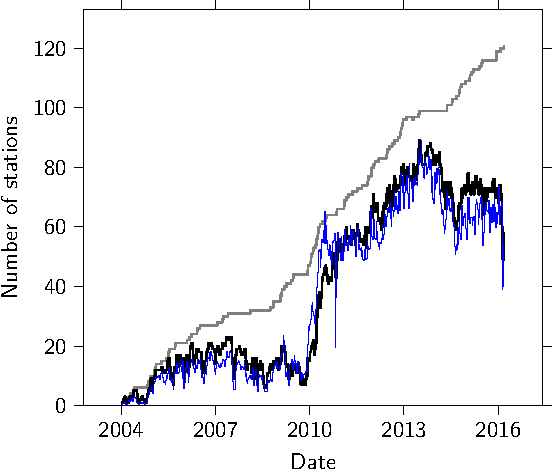
\includegraphics[width=0.6\textwidth]
                    {plots/cluster/active_stations}
    \caption{Cumulative number of stations with at least an hour of good data and the number of active stations per day.}
    \label{fig:active_stations}
\end{figure}

% Each station submits data/triggered events to central datastore
When a station records data is uploads it to the central datastore at \nikhef. Here further offline analysis is performed and the data is made available for download. The automatic data analysis that is performed is described in [a later chapter]. The data is sent from the station as a HTTP POST request to the datastore server. This server checks the station number and password for verification and if all data is correctly uploaded using a checksum. If this succeeds the data is stored in the raw datastore. The datastore stores the detected events, comparator data, configuration settings, error messages, single rates, and \gps signal information. Additionally a station may upload weather data, for which the data, configuration and errors are stored. In \cref{fig:luminosity_network} the cumulative number of detected events (green) and verified good events (black) are shown.

\begin{figure}
    \centering
    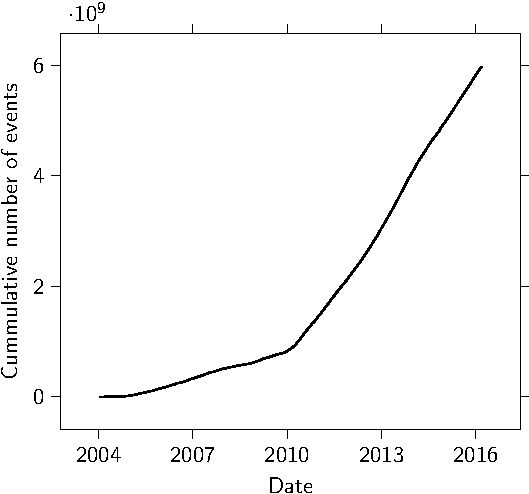
\includegraphics[width=0.6\textwidth]
                    {plots/cluster/luminosity_network}
    \caption{Cumulative number of events by all stations, the lower line contains only events when the stations were working properly.}
    \label{fig:luminosity_network}
\end{figure}

% Use offline analysis to find station events detecting the same shower.
  % - This requires good absolute timing at the stations.
  % - Use GPS at stations for both positioning of the stations (\SI{~1}{\meter}) and absolute timing (\SI{~5}{\ns}).
An `offline trigger' is used to determine when stations were probably detecting the same shower. This is similar to the station trigger. In this case the data is searched for (at least two) stations that simultaneously (i.e. within a certain time window) detected events. These events that are likely due to the same shower are called coincidences. Coincidences between stations are expect to be caused by either the detection of the same shower, the detection of separate but correlated showers (due to the GZ-effect), or the detection of two unrelated showers.

The absolute timing of events detected by stations is important when looking for coincidences. It also influences the resolution with which coincidences can be reconstructed, because the arrival times in the detectors of the stations is to be compared. The \gps of each station provides accurate absolute timing. When the station is first deployed the \gps will determine its location for \SI{24}{\hour}. After this the \gps will enter the so called `Overdetermined Clock' mode. In this mode the \gps keeps it position fixed and only concerns itself with timing. When properly processed this results in a timing accuracy of \SI{5}{\ns}.

\subsection{Station locations}

% Current station locations, explain why the stations are in those locations. Due to those being the locations of high schools..
In \cref{fig:network} the locations of all \hisparc stations is shown. Most stations are clustered in or around the slightly larger cities. The locations are in most cases limited to the locations of high schools and universities. Universities provide support for the high schools in their region, they guide students in building the detectors and provide support when needed. There are currently about \num{650} high schools in the Netherlands, some of which have multiple locations, resulting in a total of about \num{1500} high-school locations. Currently there are \num{80} Dutch high schools participating in \hisparc.

\subsubsection{International}

Locations of \hisparc stations are not limited to the Netherlands. Two other countries successfully operate multiple detection stations. All station locations are shown in \cref{fig:network}.

Since 2007 there has been a \hisparc station in Denmark. There are currently 3 operational stations at the Aarhus University. These stations are managed by Uffe Amelung Fredens. Fredens also makes student materials for Danish high-school students.

In the United Kingdom a new cluster in Bristol was started in March 2012. This was initiated by Dr. Jaap Velthuis, who is the cluster coordinator for the Bristol cluster. Since then more than 10 schools around Bristol have created detectors and joined the network. Even more schools have plans to join. In 2014 a second cluster was started in the United Kingdom around Birmingham. The Birmingham cluster is coordinated by Cristina Lazzeroni.

In Germany a station (70001) was placed inside the \kascade experiment in Karlsruhe, from 2008 up to and including 2011. This was done to calibrate and test the direction reconstruction accuracy of a single \hisparc station. Although the \kascade-GRANDE experiment officially shut down on March 30, 2009, it was kept active until November, 26th 2011 as a test facility for some test setups, including our detection station. \kascade triggered the \hisparc station when it detected a shower. More than \num{9e7} triggers occurred [2010-2011 in datastore, rest in /databases/kascade] in this period. The detectors used for the \kascade station have since been repurposed and now form station 508 at the Science Park.

\begin{figure}
    \centering
    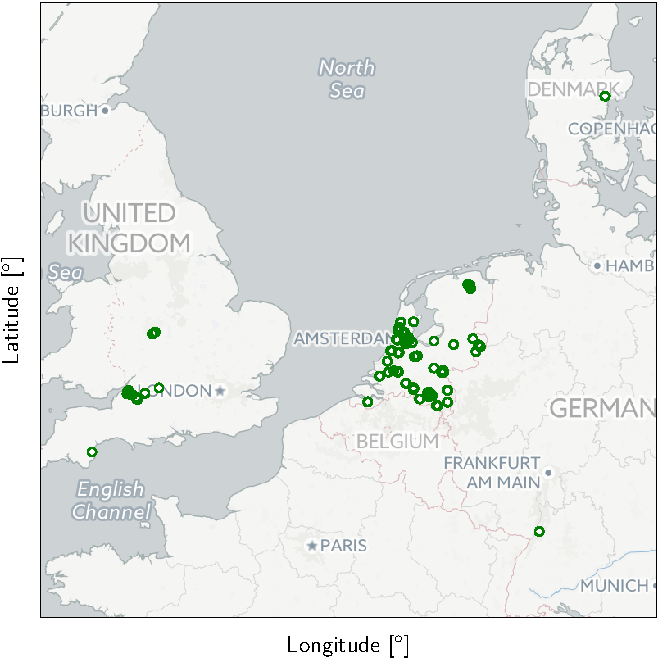
\includegraphics[width=0.6\textwidth]
                    {plots/cluster/network}
    \caption{Locations of HiSPARC stations in Netherlands, United Kingdom, and Denmark. Stations which also include a weather station are indicated with red circles.}
    \label{fig:network}
\end{figure}

Interesting for shower reconstruction, coincidence rate, and possibilities for detection the GZ-effect are the distances between pairs of stations. In \cref{fig:network_station_distances} the distribution of distances between all possible pairs of stations are shown. The points beyond \SI{250}{\kilo\meter} are due to combinations between stations in the Netherlands and the international stations. And the pair separated by only \SI{2}{\meter} is the combination of station 501 and 510. These were specifically placed to compare the results from two stations which are virtually at the same location. The results from comparing these stations is shown in [ref to later chapter about station performance or reconstructions].

\begin{figure}
    \centering
    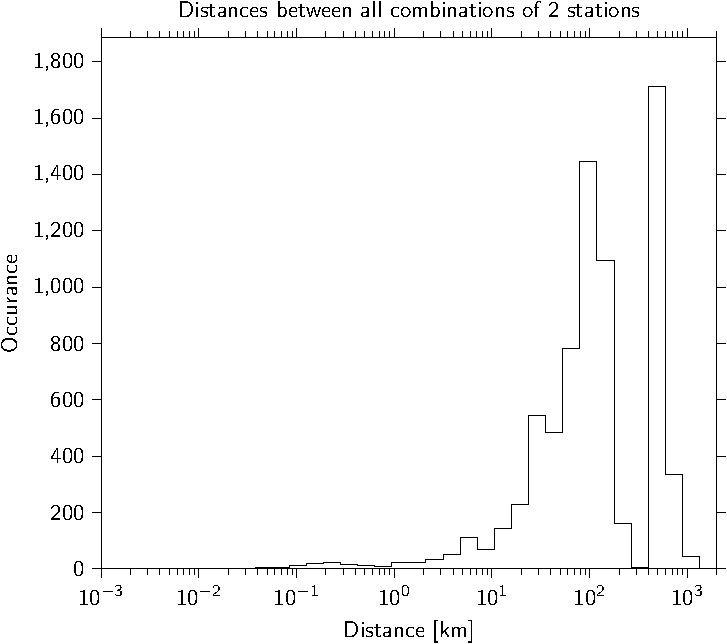
\includegraphics[width=0.6\textwidth]
                    {plots/cluster/network_station_distances}
    \caption{Distribution of distances between all possible pairs of stations in the entire HiSPARC network.}
    \label{fig:network_station_distances}
\end{figure}

\subsection{Coincidence rate}

% Stations closer than \SI{2e3}{\meter} are likely to at some point detect the same shower.
For stations up to \SI{2e3}{\meter} distance from each other they are likely to detect the same shower at some point in time. However, the rate is so low that it approaches the rate of coincidences due to random background particles. Real events may still be distinguishable from background if the event can be reconstructed very well. Large showers which can be detected efficiently by two stations both \SI{e3}{\meter} from the shower core have energies of at least \SI{e18}{\eV}. Such showers are rare, from \cref{fig:spectrum} we can estimate a rate of approximately \SI{1}{\per\kilo\meter\squared\per\day}. The sensitivity to those showers is not equal over that \si{\kilo\meter\squared} area, so a lower rate is expected.

% estimate the coincidence rate for showers of certain energy.
As the distance between stations increase the probability of detecting low energy showers decrease. The highest contributions to coincidences are the lowest energy showers that can still be detected efficiently. This smoothly transitions to continually higher showers being the dominant source for coincidences. A rough estimate can be made by using the methods described above. For detector stations at a given distance calculate the probability of detecting showers for all relevant energies in the cosmic-ray spectrum (\SIrange{e13}{e20}{\eV}). Assume that the shower hit precisely between the stations, where the probability is highest. Scale the determined probability of detection with the occurrence of such showers and compensate for the larger effective area for which high energy showers will be detectable.

In \cref{fig:distance_v_coincidence_rate} the coincidence rate is determined for all pairs of stations. Counting only the time that both stations were working properly. The determined coincidence rate is then plotted against the distance between the stations. Different coincidence rates due to detection efficiencies caused by the different number of detectors in stations is expected. The different combinations of two 2-detector, two 4-detector, and a 2- and 4-detector stations are indicated by different symbols. The background rate is estimated by \cref{eq:background_rate} and indicated by the horizontal dashed lines. A set of station pairs to far apart (\SI{>9}{\kilo\meter}) to expect coincidences is also shown to verify the background rates.

\begin{figure}
    \centering
    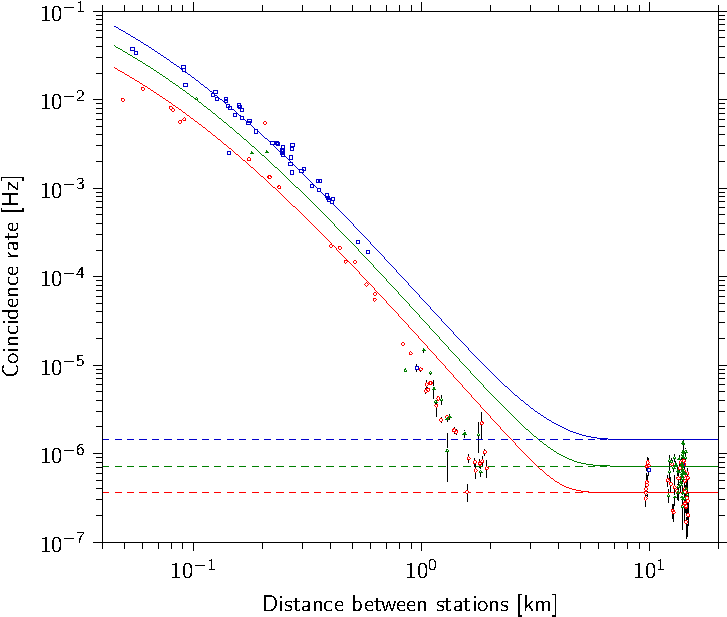
\includegraphics[width=0.6\textwidth]
                    {plots/cluster/distance_v_coincidence_rate}
    \caption{Coincidence rate between stations as a function of distance. At increasing distances the contributions from increasingly larger/energetic showers dominate. The background rate is also shown (dashed). Real events may still be distinguished from background. The square indicates two 4-detector stations, triangle for a 4- and 2-detector station, and the circle two 2-detector stations.}
    \label{fig:distance_v_coincidence_rate}
\end{figure}

\subsection{Shower reconstruction with multiple stations}

% Similar direction reconstruction algorithm as used for single station.
With the combined measurement data from multiple stations a more accurate reconstruction is possible. The distances between the detection points are larger while the timing accuracy remains excellent. The reconstruction algorithm needs to take into account the different relative altitudes of the detectors, since these are no longer all at the same altitudes \cite{steijger2012direction}. Note that for some stations (e.g. 507 and 1009) the detectors are also not all at the same altitude, but that is very rare. The Cartesian approach is used for 3D reconstruction of the shower direction \cite{montanus2015direction}

\begin{equation}
    \label{eq:direction3dflat}
    \begin{split}
        \phi &= \arctan \left(\frac{(\mathbf{u} \times \mathbf{v})_y \pm v_y \sqrt{v^2-u^2}}{(\mathbf{u} \times \mathbf{v})_x \pm v_x \sqrt{v^2-u^2}}\right) \ , \\
        \theta & = \arccos \left( \frac{(\mathbf{u} \times \mathbf{v})_z \pm v_z \sqrt{v^2-u^2}}{v^2}\right) \ .
    \end{split}
\end{equation}

Where ....[explain terms].

% At large core distances the curvature of the shower front should be taken into account.
Moreover, the curvature and rise time of the shower front play a big role and need to be accounted for in the reconstruction.

% For a large event should arrival times in each detector be used or station average density and average/first arrival time?
For stations separated by large distances the reconstruction can be performed using data from all individual detectors in each station or by using a station average. It depends on the used reconstruction algorithm what the best choice will be. In case of using the first arrival time from all detectors at the station arrival time will provide better results for a reconstruction assuming a flat shower front. In the case of a shaped shower front the reconstruction should take into account the probability of detection and thus the most likely arrival times. For arrival direction reconstruction using a shaped shower front the shower axis (core) location must be known. In \cref{fig:angle_between_501_minn16_510} reconstruction accuracy using the individual detector arrival times is compared to a reconstruction using station averages (or first?).

\begin{figure}
    \centering
    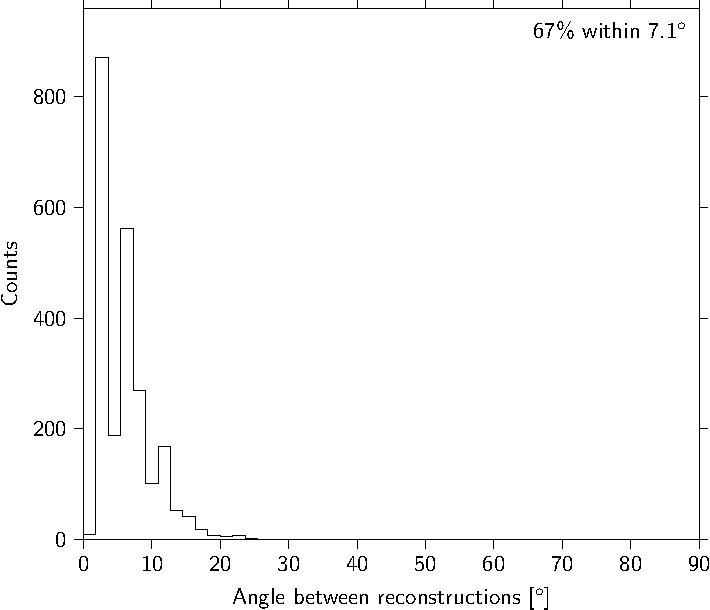
\includegraphics[width=0.6\textwidth]
                    {plots/cluster/angle_between_501_minn16_510}
    \caption{(placeholder plot, not data mentioned in caption) Distance between reconstructions when using average/first arrival time, versus simulation input. Using separate detectors should hold more information, but the reconstruction algorithm should be aware (using curved or flat reconstruction?)}
    \label{fig:angle_between_501_minn16_510}
\end{figure}


\section{Positions}

\subsection{\gps Self-Survey}

To get a fix on the position of a stationary \gps antenna the \gps can perform a self-survey. During the self-survey the \gps will continuously determine its location, at the end of the survey the center of the clouds of positions will be taken as the correct location. \gps satellites orbit the Earth every \SI{12}{\hour}, taking in account the rotation of the Earth the \gps satellites will be above the same location of the Earth every \SI{24}{\hour}. The positions of the \gps satellites has an effect on the accuracy of the \gps, this is shown in ...(bad position -> periodic offsets). By using a self-survey of \SI{86400}{\second} (i.e. \SI{24}{\hour}) a good average is determined, which should minimize the time error. Normally this self-survey needs to be performed only once, if the \gps remains fixed in its place. In order to guess the accuracy of the self-survey it has been performed multiple times for some stations to see the spread in the results.

Two \gps antennae separated by \SI{2}{\meter} are used by station 501 and station 510. Each station performed a self-survey with its own \gps and one with the \gps of the other station to test the accuracy.

\begin{verbatim}
GPS s510
s510  1412347130	52.3558955	4.9509864	54.59
s501  1414406502	52.3558990	4.9509880	57.65

GPS s501
s501  1412347557	52.3558800	4.9510065	55.40
s510  1414406952	52.3558859	4.9510083	57.39
\end{verbatim}

Difference of \SI{1.}{\centi\meter}, but \SI{2}{\meter} in altitude.

Looking at the available gps positions see a spread of 2 meters, but possibly contaminated by short surveys.


\section{Timing}

\subsection{\gps timestamp, electronics}

When considering coincidences between stations the accuracy of the timing is crucial, both for correctly identifying coincidences and for the reconstruction. Similar to the offsets between detectors in a station, offsets between stations have been found. These may be caused by different detector cable lengths, \gps antennae cable length, and possibly something in the electronics of the \hisparc box.

Determining the station offset requires many coincidences. The number of coincidences between stations is inversely correlated to the the distance between them. Moreover the width of the $\Delta t$ distribution between stations is dominated by time differences due to the arrival direction of the showers. This time difference increases with distance, if the azimuth direction is along the line between the stations then $\Delta t = r \sin{\theta}$. The distance between stations negatively affects the number of coincidences and increases the width of the $\Delta t$ distribution, making it harder to precisely determine the average offset. However, when distances become very large the accuracy of the offset will be less important, because it will have a smaller effect on the direction of the shower.

\begin{figure}
    \centering
    % \usepackage{tikz}
% \usetikzlibrary{arrows,external}
% \usepackage{pgfplots}
% \pgfplotsset{compat=1.3}
% \usepackage[detect-family]{siunitx}
% \usepackage[eulergreek]{sansmath}
% \sisetup{text-sf=\sansmath}
% \usepackage{relsize}
%
    \tikzsetnextfilename{externalized-station_offsets_501_502}
\pgfkeysifdefined{/artist/width}
    {\pgfkeysgetvalue{/artist/width}{\defaultwidth}}
    {\def\defaultwidth{ .67\linewidth }}
%
%
\begin{sansmath}
\begin{tikzpicture}[
        font=\sffamily,
        every pin/.style={inner sep=2pt, font={\sffamily\smaller}},
        every label/.style={inner sep=2pt, font={\sffamily\smaller}},
        every pin edge/.style={<-, >=stealth', shorten <=2pt},
        pin distance=2.5ex,
    ]
    \begin{axis}[
            axis background/.style={  },
            xmode=normal,
            ymode=normal,
            width=\defaultwidth,
            scale only axis,
            axis equal=false,
            %
            title={  },
            %
            xlabel={ $\Delta t$ [ns] },
            ylabel={ Counts },
            %
            xmin={ -454.427641037 },
            xmax={ 454.427641037 },
            ymin={ 0 },
            ymax={  },
            %
            xtick={  },
            ytick={  },
            %
            tick align=outside,
            max space between ticks=40,
            every tick/.style={},
            axis on top,
            point meta min={  },
            point meta max={  },
                colormap={coolwarm}{
                    rgb255(0cm)=( 59, 76,192);
                    rgb255(1cm)=( 98,130,234);
                    rgb255(2cm)=(141,176,254);
                    rgb255(3cm)=(184,208,249);
                    rgb255(4cm)=(221,221,221);
                    rgb255(5cm)=(245,196,173);
                    rgb255(6cm)=(244,154,123);
                    rgb255(7cm)=(222, 96, 77);
                    rgb255(8cm)=(180,  4, 38)},
        ]

        


    
    % Draw series plot
    \addplot[no markers,gray] coordinates {
            (-451.377791098, 0.114273479435)
            (-445.278091218, 0.149888768534)
            (-439.178391338, 0.195867290975)
            (-433.078691459, 0.254990456595)
            (-426.978991579, 0.330715935102)
            (-420.879291699, 0.42732224444)
            (-414.779591819, 0.550078999416)
            (-408.67989194, 0.70544606297)
            (-402.58019206, 0.901304932575)
            (-396.48049218, 1.14722569724)
            (-390.380792301, 1.45477279097)
            (-384.281092421, 1.83785251871)
            (-378.181392541, 2.31310491114)
            (-372.081692662, 2.90034184411)
            (-365.981992782, 3.62303250754)
            (-359.882292902, 4.5088361966)
            (-353.782593022, 5.59018100119)
            (-347.682893143, 6.90488526629)
            (-341.583193263, 8.49681667426)
            (-335.483493383, 10.416581457)
            (-329.383793504, 12.722233593)
            (-323.284093624, 15.4799909056)
            (-317.184393744, 18.7649418002)
            (-311.084693865, 22.6617230195)
            (-304.984993985, 27.2651453499)
            (-298.885294105, 32.6807407749)
            (-292.785594225, 39.0252012885)
            (-286.685894346, 46.4266765905)
            (-280.586194466, 55.024895371)
            (-274.486494586, 64.9710730265)
            (-268.386794707, 76.427567649)
            (-262.287094827, 89.5672461749)
            (-256.187394947, 104.572523879)
            (-250.087695068, 121.634043131)
            (-243.987995188, 140.948961641)
            (-237.888295308, 162.718826452)
            (-231.788595428, 187.147017703)
            (-225.688895549, 214.435755801)
            (-219.589195669, 244.782676884)
            (-213.489495789, 278.37699439)
            (-207.38979591, 315.395278741)
            (-201.29009603, 355.996902443)
            (-195.19039615, 400.319213855)
            (-189.090696271, 448.472518925)
            (-182.990996391, 500.534965935)
            (-176.891296511, 556.547442963)
            (-170.791596632, 616.508610845)
            (-164.691896752, 680.370205109)
            (-158.592196872, 748.032748146)
            (-152.492496992, 819.341817017)
            (-146.392797113, 894.085012344)
            (-140.293097233, 971.989769214)
            (-134.193397353, 1052.72214163)
            (-128.093697474, 1135.88667762)
            (-121.993997594, 1221.02748283)
            (-115.894297714, 1307.63054625)
            (-109.794597835, 1395.12737326)
            (-103.694897955, 1482.89993954)
            (-97.5951980752, 1570.28694396)
            (-91.4954981955, 1656.59130252)
            (-85.3957983158, 1741.08878769)
            (-79.2960984361, 1823.0376812)
            (-73.1963985564, 1901.68927318)
            (-67.0966986767, 1976.29900939)
            (-60.996998797, 2046.13806088)
            (-54.8972989173, 2110.50506918)
            (-48.7975990376, 2168.73780517)
            (-42.6978991579, 2220.22447243)
            (-36.5981992782, 2264.41438629)
            (-30.4984993985, 2300.8277684)
            (-24.3987995188, 2329.06441368)
            (-18.2990996391, 2348.81101055)
            (-12.1993997594, 2359.84692758)
            (-6.0996998797, 2362.04831687)
            (2.84217094304e-14, 2355.39042758)
            (6.0996998797, 2339.94806916)
            (12.1993997594, 2315.89421211)
            (18.2990996391, 2283.49676301)
            (24.3987995188, 2243.1135976)
            (30.4984993985, 2195.18598109)
            (36.5981992782, 2140.23054439)
            (42.6978991579, 2078.83002048)
            (48.7975990376, 2011.62297301)
            (54.8972989173, 1939.29276967)
            (60.996998797, 1862.55606612)
            (67.0966986767, 1782.15107027)
            (73.1963985564, 1698.82585347)
            (79.2960984361, 1613.32696387)
            (85.3957983158, 1526.38857878)
            (91.4954981955, 1438.72240869)
            (97.5951980752, 1351.00853582)
            (103.694897955, 1263.88733721)
            (109.794597835, 1177.95260579)
            (115.894297714, 1093.74594653)
            (121.993997594, 1011.75248694)
            (128.093697474, 932.397905823)
            (134.193397353, 856.046750443)
            (140.293097233, 783.001982033)
            (146.392797113, 713.505663238)
            (152.492496992, 647.740679398)
            (158.592196872, 585.833368649)
            (164.691896752, 527.85692395)
            (170.791596632, 473.835423265)
            (176.891296511, 423.748341892)
            (182.990996391, 377.535403183)
            (189.090696271, 335.10162986)
            (195.19039615, 296.32246753)
            (201.29009603, 261.048863943)
            (207.38979591, 229.112201498)
            (213.489495789, 200.328995802)
            (219.589195669, 174.505289038)
            (225.688895549, 151.440682982)
            (231.788595428, 130.931972173)
            (237.888295308, 112.776352509)
            (243.987995188, 96.7741941765)
            (250.087695068, 82.7313798703)
            (256.187394947, 70.4612197523)
            (262.287094827, 59.7859632398)
            (268.386794707, 50.5379346297)
            (274.486494586, 42.5603247043)
            (280.586194466, 35.7076739676)
            (286.685894346, 29.846085146)
            (292.785594225, 24.8532032363)
            (298.885294105, 20.6180008731)
            (304.984993985, 17.0404053302)
            (311.084693865, 14.0308012513)
            (317.184393744, 11.5094404321)
            (323.284093624, 9.40578681354)
            (329.383793504, 7.65782147114)
            (335.483493383, 6.21132892698)
            (341.583193263, 5.01918269665)
            (347.682893143, 4.04064470724)
            (353.782593022, 3.24069015729)
            (359.882292902, 2.58936659058)
            (365.981992782, 2.06119345657)
            (372.081692662, 1.63460624856)
            (378.181392541, 1.29144745027)
            (384.281092421, 1.0165049747)
            (390.380792301, 0.797097528149)
            (396.48049218, 0.622705355883)
            (402.58019206, 0.484644093928)
            (408.67989194, 0.37577893643)
            (414.779591819, 0.290275997379)
            (420.879291699, 0.223387569931)
            (426.978991579, 0.171267936959)
            (433.078691459, 0.13081643625)
            (439.178391338, 0.0995446091852)
            (445.278091218, 0.0754644415944)
            (451.377791098, 0.0569949221089)
    };

    
    % Draw series plot
    \addplot[no markers,solid,const plot] coordinates {
            (-454.427641037, 3)
            (-448.327941158, 3)
            (-442.228241278, 0)
            (-436.128541398, 3)
            (-430.028841519, 0)
            (-423.929141639, 6)
            (-417.829441759, 6)
            (-411.72974188, 0)
            (-405.630042, 0)
            (-399.53034212, 6)
            (-393.43064224, 3)
            (-387.330942361, 0)
            (-381.231242481, 12)
            (-375.131542601, 0)
            (-369.031842722, 3)
            (-362.932142842, 6)
            (-356.832442962, 3)
            (-350.732743083, 6)
            (-344.633043203, 0)
            (-338.533343323, 12)
            (-332.433643443, 15)
            (-326.333943564, 12)
            (-320.234243684, 12)
            (-314.134543804, 9)
            (-308.034843925, 15)
            (-301.935144045, 21)
            (-295.835444165, 0)
            (-289.735744286, 30)
            (-283.636044406, 24)
            (-277.536344526, 39)
            (-271.436644647, 39)
            (-265.336944767, 39)
            (-259.237244887, 51)
            (-253.137545007, 60)
            (-247.037845128, 60)
            (-240.938145248, 90)
            (-234.838445368, 174)
            (-228.738745489, 183)
            (-222.639045609, 198)
            (-216.539345729, 213)
            (-210.43964585, 270)
            (-204.33994597, 300)
            (-198.24024609, 378)
            (-192.14054621, 414)
            (-186.040846331, 465)
            (-179.941146451, 543)
            (-173.841446571, 717)
            (-167.741746692, 801)
            (-161.642046812, 729)
            (-155.542346932, 789)
            (-149.442647053, 828)
            (-143.342947173, 975)
            (-137.243247293, 1083)
            (-131.143547413, 1143)
            (-125.043847534, 1377)
            (-118.944147654, 1392)
            (-112.844447774, 1356)
            (-106.744747895, 1455)
            (-100.645048015, 1623)
            (-94.5453481353, 1899)
            (-88.4456482556, 1710)
            (-82.3459483759, 1848)
            (-76.2462484962, 1761)
            (-70.1465486165, 2124)
            (-64.0468487368, 2073)
            (-57.9471488571, 2091)
            (-51.8474489774, 2118)
            (-45.7477490977, 2139)
            (-39.648049218, 2145)
            (-33.5483493383, 2235)
            (-27.4486494586, 2460)
            (-21.3489495789, 2397)
            (-15.2492496992, 2148)
            (-9.14954981955, 2451)
            (-3.04984993985, 2226)
            (3.04984993985, 2454)
            (9.14954981955, 2214)
            (15.2492496992, 2244)
            (21.3489495789, 2124)
            (27.4486494586, 2118)
            (33.5483493383, 2166)
            (39.648049218, 2160)
            (45.7477490977, 2121)
            (51.8474489774, 1827)
            (57.9471488571, 2025)
            (64.0468487368, 1737)
            (70.1465486165, 1644)
            (76.2462484962, 1548)
            (82.3459483759, 1632)
            (88.4456482556, 1536)
            (94.5453481353, 1404)
            (100.645048015, 1311)
            (106.744747895, 1191)
            (112.844447774, 1137)
            (118.944147654, 1080)
            (125.043847534, 993)
            (131.143547413, 867)
            (137.243247293, 825)
            (143.342947173, 711)
            (149.442647053, 705)
            (155.542346932, 621)
            (161.642046812, 474)
            (167.741746692, 459)
            (173.841446571, 372)
            (179.941146451, 333)
            (186.040846331, 246)
            (192.14054621, 204)
            (198.24024609, 219)
            (204.33994597, 186)
            (210.43964585, 102)
            (216.539345729, 108)
            (222.639045609, 78)
            (228.738745489, 90)
            (234.838445368, 78)
            (240.938145248, 57)
            (247.037845128, 63)
            (253.137545007, 36)
            (259.237244887, 21)
            (265.336944767, 36)
            (271.436644647, 18)
            (277.536344526, 27)
            (283.636044406, 9)
            (289.735744286, 15)
            (295.835444165, 9)
            (301.935144045, 15)
            (308.034843925, 6)
            (314.134543804, 0)
            (320.234243684, 3)
            (326.333943564, 3)
            (332.433643443, 3)
            (338.533343323, 3)
            (344.633043203, 6)
            (350.732743083, 6)
            (356.832442962, 9)
            (362.932142842, 6)
            (369.031842722, 3)
            (375.131542601, 0)
            (381.231242481, 0)
            (387.330942361, 0)
            (393.43064224, 0)
            (399.53034212, 6)
            (405.630042, 3)
            (411.72974188, 0)
            (417.829441759, 0)
            (423.929141639, 3)
            (430.028841519, 6)
            (436.128541398, 0)
            (442.228241278, 3)
            (448.327941158, 6)
            (454.427641037, 6)
    };

    \node[,
          below left=2pt
        ]
        at (rel axis cs:1,1)
        { $\mu$: -7.63, $\sigma$: 99.54 };

    \end{axis}
\end{tikzpicture}
\end{sansmath}

    \caption{\captitle{Coincidence time difference distribution.} The
             time difference between events in coincidence detected by
             station 501 and 502 in a three week period in 2010. The
             width of the distribution is caused by the distance between
             stations and showers under angles.}
    \label{fig:station_offsets_501_502}
\end{figure}

\begin{figure}
    \centering
    % \usepackage{tikz}
% \usetikzlibrary{arrows,external}
% \usepackage{pgfplots}
% \pgfplotsset{compat=1.3}
% \usepackage[detect-family]{siunitx}
% \usepackage[eulergreek]{sansmath}
% \sisetup{text-sf=\sansmath}
% \usepackage{relsize}
%
    \tikzsetnextfilename{externalized-station_offsets_501_510}
\pgfkeysifdefined{/artist/width}
    {\pgfkeysgetvalue{/artist/width}{\defaultwidth}}
    {\def\defaultwidth{ .67\linewidth }}
%
%
\begin{sansmath}
\begin{tikzpicture}[
        font=\sffamily,
        every pin/.style={inner sep=2pt, font={\sffamily\smaller}},
        every label/.style={inner sep=2pt, font={\sffamily\smaller}},
        every pin edge/.style={<-, >=stealth', shorten <=2pt},
        pin distance=2.5ex,
    ]
    \begin{axis}[
            axis background/.style={  },
            xmode=normal,
            ymode=normal,
            width=\defaultwidth,
            scale only axis,
            axis equal=false,
            %
            title={  },
            %
            xlabel={ $\Delta t$ [ns] },
            ylabel={ Counts },
            %
            xmin={ -150.0 },
            xmax={ 150.0 },
            ymin={ 0 },
            ymax={  },
            %
            xtick={  },
            ytick={  },
            %
            tick align=outside,
            max space between ticks=40,
            every tick/.style={},
            axis on top,
            point meta min={  },
            point meta max={  },
                colormap={coolwarm}{
                    rgb255(0cm)=( 59, 76,192);
                    rgb255(1cm)=( 98,130,234);
                    rgb255(2cm)=(141,176,254);
                    rgb255(3cm)=(184,208,249);
                    rgb255(4cm)=(221,221,221);
                    rgb255(5cm)=(245,196,173);
                    rgb255(6cm)=(244,154,123);
                    rgb255(7cm)=(222, 96, 77);
                    rgb255(8cm)=(180,  4, 38)},
        ]

        


    
    % Draw series plot
    \addplot[no markers,gray] coordinates {
            (-148.993288591, 7.98951572119e-19)
            (-146.979865772, 9.13828681033e-18)
            (-144.966442953, 9.83870217454e-17)
            (-142.953020134, 9.97101902943e-16)
            (-140.939597315, 9.51195915727e-15)
            (-138.926174497, 8.54140096073e-14)
            (-136.912751678, 7.21966328527e-13)
            (-134.899328859, 5.7442519161e-12)
            (-132.88590604, 4.3020822906e-11)
            (-130.872483221, 3.03286200145e-10)
            (-128.859060403, 2.01258989297e-09)
            (-126.845637584, 1.25714862825e-08)
            (-124.832214765, 7.39173970731e-08)
            (-122.818791946, 4.09105582359e-07)
            (-120.805369128, 2.13134054612e-06)
            (-118.791946309, 1.04519900887e-05)
            (-116.77852349, 4.82473908711e-05)
            (-114.765100671, 0.000209641557076)
            (-112.751677852, 0.000857451613395)
            (-110.738255034, 0.00330119035817)
            (-108.724832215, 0.011963554024)
            (-106.711409396, 0.0408111246639)
            (-104.697986577, 0.131046556086)
            (-102.684563758, 0.396096825795)
            (-100.67114094, 1.12695302343)
            (-98.6577181208, 3.0181371073)
            (-96.644295302, 7.60853105855)
            (-94.6308724832, 18.054745525)
            (-92.6174496644, 40.3283660434)
            (-90.6040268456, 84.7927229674)
            (-88.5906040268, 167.816723971)
            (-86.5771812081, 312.637159641)
            (-84.5637583893, 548.244968985)
            (-82.5503355705, 904.976735049)
            (-80.5369127517, 1406.14101173)
            (-78.5234899329, 2056.59623597)
            (-76.5100671141, 2831.37829873)
            (-74.4966442953, 3669.23445065)
            (-72.4832214765, 4475.91393214)
            (-70.4697986577, 5139.4505545)
            (-68.4563758389, 5554.95261233)
            (-66.4429530201, 5651.61703761)
            (-64.4295302013, 5412.44871042)
            (-62.4161073826, 4879.14318301)
            (-60.4026845638, 4140.20678933)
            (-58.389261745, 3306.96199838)
            (-56.3758389262, 2486.36610287)
            (-54.3624161074, 1759.66359568)
            (-52.3489932886, 1172.25723902)
            (-50.3355704698, 735.09741957)
            (-48.322147651, 433.905918655)
            (-46.3087248322, 241.087642935)
            (-44.2953020134, 126.090692171)
            (-42.2818791946, 62.0754401375)
            (-40.2684563758, 28.7663849111)
            (-38.255033557, 12.5481432495)
            (-36.2416107383, 5.15231432058)
            (-34.2281879195, 1.9913790423)
            (-32.2147651007, 0.724493036815)
            (-30.2013422819, 0.248109389609)
            (-28.1879194631, 0.0799799053391)
            (-26.1744966443, 0.0242687424192)
            (-24.1610738255, 0.00693174151748)
            (-22.1476510067, 0.00186365769995)
            (-20.1342281879, 0.000471648695211)
            (-18.1208053691, 0.000112356920537)
            (-16.1073825503, 2.51947305956e-05)
            (-14.0939597315, 5.3179997314e-06)
            (-12.0805369128, 1.05661215945e-06)
            (-10.067114094, 1.97611219527e-07)
            (-8.05369127517, 3.47885472659e-08)
            (-6.04026845638, 5.76487227308e-09)
            (-4.02684563758, 8.99232068769e-10)
            (-2.01342281879, 1.32033028331e-10)
            (1.42108547152e-14, 1.82482861882e-11)
            (2.01342281879, 2.37405230596e-12)
            (4.02684563758, 2.90728216514e-13)
            (6.04026845638, 3.35129598248e-14)
            (8.05369127517, 3.63636181519e-15)
            (10.067114094, 3.71407006544e-16)
            (12.0805369128, 3.57076933978e-17)
            (14.0939597315, 3.23148543434e-18)
            (16.1073825503, 2.75277876405e-19)
            (18.1208053691, 2.20733940796e-20)
            (20.1342281879, 1.66607913437e-21)
            (22.1476510067, 1.18372504083e-22)
            (24.1610738255, 7.91652787542e-24)
            (26.1744966443, 4.98364796153e-25)
            (28.1879194631, 2.9531715037e-26)
            (30.2013422819, 1.64724683745e-27)
            (32.2147651007, 8.64883071552e-29)
            (34.2281879195, 4.27449498554e-30)
            (36.2416107383, 1.98857020548e-31)
            (38.255033557, 8.70814687288e-33)
            (40.2684563758, 3.58954385304e-34)
            (42.2818791946, 1.39277666705e-35)
            (44.2953020134, 5.08689065703e-37)
            (46.3087248322, 1.74884783433e-38)
            (48.322147651, 5.65952972823e-40)
            (50.3355704698, 1.72400042454e-41)
            (52.3489932886, 4.94336971184e-43)
            (54.3624161074, 1.33425093912e-44)
            (56.3758389262, 3.38985126252e-46)
            (58.389261745, 8.10685620335e-48)
            (60.4026845638, 1.82495851889e-49)
            (62.4161073826, 3.86707171467e-51)
            (64.4295302013, 7.71329880438e-53)
            (66.4429530201, 1.44819414183e-54)
            (68.4563758389, 2.55942329199e-56)
            (70.4697986577, 4.25780875304e-58)
            (72.4832214765, 6.66743643424e-60)
            (74.4966442953, 9.82789071115e-62)
            (76.5100671141, 1.36361086755e-63)
            (78.5234899329, 1.78094000748e-65)
            (80.5369127517, 2.18945905279e-67)
            (82.5503355705, 2.53368759854e-69)
            (84.5637583893, 2.75992960439e-71)
            (86.5771812081, 2.82990362295e-73)
            (88.5906040268, 2.7313288141e-75)
            (90.6040268456, 2.48144714105e-77)
            (92.6174496644, 2.12209475284e-79)
            (94.6308724832, 1.70825702568e-81)
            (96.644295302, 1.29440553261e-83)
            (98.6577181208, 9.23243388995e-86)
            (100.67114094, 6.19855920135e-88)
            (102.684563758, 3.91736466211e-90)
            (104.697986577, 2.33037573816e-92)
            (106.711409396, 1.30492815026e-94)
            (108.724832215, 6.87821822741e-97)
            (110.738255034, 3.41266770334e-99)
            (112.751677852, 1.59382544191e-101)
            (114.765100671, 7.00674332942e-104)
            (116.77852349, 2.89948164178e-106)
            (118.791946309, 1.1294141353e-108)
            (120.805369128, 4.14109101173e-111)
            (122.818791946, 1.42923957425e-113)
            (124.832214765, 4.64327056959e-116)
            (126.845637584, 1.41994541827e-118)
            (128.859060403, 4.08740819262e-121)
            (130.872483221, 1.10752381194e-123)
            (132.88590604, 2.82479434199e-126)
            (134.899328859, 6.78186745885e-129)
            (136.912751678, 1.53264108055e-131)
            (138.926174497, 3.26032074435e-134)
            (140.939597315, 6.52843212787e-137)
            (142.953020134, 1.23051287023e-139)
            (144.966442953, 2.1831929915e-142)
            (146.979865772, 3.64608507121e-145)
            (148.993288591, 5.73178864069e-148)
    };

    
    % Draw series plot
    \addplot[no markers,solid,const plot] coordinates {
            (-150.0, 5)
            (-147.986577181, 1)
            (-145.973154362, 3)
            (-143.959731544, 8)
            (-141.946308725, 8)
            (-139.932885906, 2)
            (-137.919463087, 10)
            (-135.906040268, 11)
            (-133.89261745, 5)
            (-131.879194631, 12)
            (-129.865771812, 7)
            (-127.852348993, 7)
            (-125.838926174, 12)
            (-123.825503356, 9)
            (-121.812080537, 14)
            (-119.798657718, 11)
            (-117.785234899, 14)
            (-115.771812081, 29)
            (-113.758389262, 26)
            (-111.744966443, 34)
            (-109.731543624, 38)
            (-107.718120805, 49)
            (-105.704697987, 68)
            (-103.691275168, 77)
            (-101.677852349, 86)
            (-99.6644295302, 115)
            (-97.6510067114, 172)
            (-95.6375838926, 217)
            (-93.6241610738, 279)
            (-91.610738255, 364)
            (-89.5973154362, 457)
            (-87.5838926174, 618)
            (-85.5704697987, 794)
            (-83.5570469799, 1097)
            (-81.5436241611, 1360)
            (-79.5302013423, 1961)
            (-77.5167785235, 2595)
            (-75.5033557047, 3438)
            (-73.4899328859, 4402)
            (-71.4765100671, 5194)
            (-69.4630872483, 5768)
            (-67.4496644295, 5752)
            (-65.4362416107, 5582)
            (-63.4228187919, 4727)
            (-61.4093959732, 4398)
            (-59.3959731544, 2908)
            (-57.3825503356, 2286)
            (-55.3691275168, 1668)
            (-53.355704698, 1178)
            (-51.3422818792, 852)
            (-49.3288590604, 649)
            (-47.3154362416, 540)
            (-45.3020134228, 468)
            (-43.288590604, 282)
            (-41.2751677852, 235)
            (-39.2617449664, 182)
            (-37.2483221477, 146)
            (-35.2348993289, 113)
            (-33.2214765101, 95)
            (-31.2080536913, 79)
            (-29.1946308725, 86)
            (-27.1812080537, 63)
            (-25.1677852349, 66)
            (-23.1543624161, 71)
            (-21.1409395973, 63)
            (-19.1275167785, 71)
            (-17.1140939597, 94)
            (-15.1006711409, 97)
            (-13.0872483221, 135)
            (-11.0738255034, 150)
            (-9.06040268456, 242)
            (-7.04697986577, 289)
            (-5.03355704698, 379)
            (-3.02013422819, 566)
            (-1.0067114094, 688)
            (1.0067114094, 884)
            (3.02013422819, 1075)
            (5.03355704698, 1240)
            (7.04697986577, 1292)
            (9.06040268456, 1292)
            (11.0738255034, 1090)
            (13.0872483221, 1071)
            (15.1006711409, 640)
            (17.1140939597, 513)
            (19.1275167785, 370)
            (21.1409395973, 273)
            (23.1543624161, 197)
            (25.1677852349, 159)
            (27.1812080537, 125)
            (29.1946308725, 126)
            (31.2080536913, 71)
            (33.2214765101, 49)
            (35.2348993289, 38)
            (37.2483221477, 34)
            (39.2617449664, 24)
            (41.2751677852, 15)
            (43.288590604, 17)
            (45.3020134228, 10)
            (47.3154362416, 11)
            (49.3288590604, 10)
            (51.3422818792, 7)
            (53.355704698, 6)
            (55.3691275168, 6)
            (57.3825503356, 5)
            (59.3959731544, 4)
            (61.4093959732, 7)
            (63.4228187919, 2)
            (65.4362416107, 5)
            (67.4496644295, 1)
            (69.4630872483, 4)
            (71.4765100671, 4)
            (73.4899328859, 3)
            (75.5033557047, 0)
            (77.5167785235, 4)
            (79.5302013423, 2)
            (81.5436241611, 5)
            (83.5570469799, 6)
            (85.5704697987, 0)
            (87.5838926174, 4)
            (89.5973154362, 1)
            (91.610738255, 0)
            (93.6241610738, 2)
            (95.6375838926, 1)
            (97.6510067114, 1)
            (99.6644295302, 1)
            (101.677852349, 2)
            (103.691275168, 4)
            (105.704697987, 1)
            (107.718120805, 0)
            (109.731543624, 0)
            (111.744966443, 1)
            (113.758389262, 2)
            (115.771812081, 1)
            (117.785234899, 0)
            (119.798657718, 1)
            (121.812080537, 0)
            (123.825503356, 2)
            (125.838926174, 0)
            (127.852348993, 1)
            (129.865771812, 0)
            (131.879194631, 3)
            (133.89261745, 1)
            (135.906040268, 1)
            (137.919463087, 0)
            (139.932885906, 3)
            (141.946308725, 1)
            (143.959731544, 0)
            (145.973154362, 1)
            (147.986577181, 0)
            (150.0, 0)
    };

    \node[,
          below left=2pt
        ]
        at (rel axis cs:1,1)
        { $\mu$: -66.88, $\sigma$: 8.19 };

    \end{axis}
\end{tikzpicture}
\end{sansmath}

    \caption{\captitle{Coincidence time difference distribution.} The
             time difference between events in coincidence detected by
             station 501 and 510 in a three week period in 2014. The
             width of the distribution here is caused by \gps accuracy.
             The reason for two distributions is that at some point in
             the period the \gps antennas were switched between the two
             stations.}
    \label{fig:station_offsets_501_510}
\end{figure}


\section{\gps timing accuracy}
\label{sec:gps_accuracy}

Time difference calibration measurements have been performed on HiSPARC II and III electronic boxes. This started after dr. David Fokkema discovered an unexpected time offset between timestamps of events in a test where two HiSPARC stations (501 and 502) were triggered with the same pulse generator (Fokkema 2012 p47). Since these stations are very close ($\sim\SI{100}{\meter}$) a minimal time offset was expected, any offset or large standard deviation was expected to be the result of errors in \gps accuracy and position. However, a large offset ($\Delta t \sim\SI{18}{\ns}$) was found. Further tests have been performed to determine the cause of the offset, these tests are described in this section. Both the \hisparc electronics and \gps antennas were found to have varying offsets contributing to time differences in the resulting time measurements.


\subsection{Making event timestamps}
\label{sub:gps_timestamps}

Every second the \gps receiver sends a signal (a Pulse Per Second) to the \hisparc electronics to indicate the start of a second \cite{verkooijen2008firmware}. The \hisparc box uses a $\SI{200}{\mega\hertz}$ clock to determine the time within this second. Since the crystal in this clock does not work at exactly $\SI{200}{\mega\hertz}$ the counter (reset at the arrival of a PPS) is read at the moment of an event and then when the next PPS arrives. Giving information about at what fraction of that second the event occurred. For higher accuracy (more than $\SI{5}{\ns}$) the clock is also read on the negative side of the clock, effectively making it a $\SI{400}{\mega\hertz}$ clock with $\SI{2.5}{\ns}$ accuracy. Events are sent from the \hisparc electronics to the PC as soon as they are readout, the events contain the trace data, timestamp, CTD... The extended timestamp is determined on the PC, because 3 One second messages from the electronics are required to accurately determine the extended timestamp. Determination of the extended timestamp is done with \cref{eq:timestamp}.

\begin{equation}
\label{eq:timestamp}
    Timestamp = E_{Sync} + E_{Quan1} + \left(\frac{T_{Event}}{T_{PPS}}\right)
                 \left(1e^9 - E_{Quan1} + E_{Quan2}\right)
\end{equation}

Where $E_{Quan}$ is the Quantization Error, $E_{Sync}$ is the Synchronization Error, $T_{Event}$ are the count of ticks till the event and $T_{PPS}$ are the count of ticks between the PPS before and after the event. Here the accuracy of the timestamp is improved by taking the Quantization errors into account. The quantization error for each PPS is in the following One second message. The One second message at the end of the second after the event is also required for the quantization error of the end value of the event second. The Resolution T GPS Embedded Board User Guide in correctly states this value is in seconds, it is in nanoseconds. The Synchronization Error corrects for the error made by the misalignment of the PPS and the FPGA clock.

The same procedure is done for the Master and Slave events, each using their own One second messages.


\subsection{Test setup}
\label{sub:gps_test_setup}

In the setup one \hisparc II Master (hardware serial: 62) is used as the main reference point for the entire test. All other \hisparc boxes were tested against this reference one at a time to measure the offset. Two \gps antennas ('501' and 'test') and a \gps splitter were used. With the splitter was possible to perform tests in which both \hisparc boxes used the same \gps antenna, removing the offset caused by using different \gps antennas.

Each \hisparc box was connected to a \gps antenna and a PC, each running the current version of the \hisparc Software; \hisparc DAQ II v3.0.4. When the \hisparc III boxes needed to be tested the DAQ was upgraded to the beta version of the new DAQ; \hisparc DAQ III v1.0.0.

A \SI{100}{\mega\hertz} Pulse Generator (as reference: Tabor Electronics Model 8600), with two short equal-length signal cables and a signal splitter was used to trigger the \hisparc electronics. Each box was connected to the same pulse generator through either of the PMT input channels. To ensure the generated signals arrived at the same time at the input both cables from the pulse generator were connected to the same \hisparc electronics and also switched around.

\begin{figure}
    \centering
    \tikzsetnextfilename{externalized-gps_test_setup}
 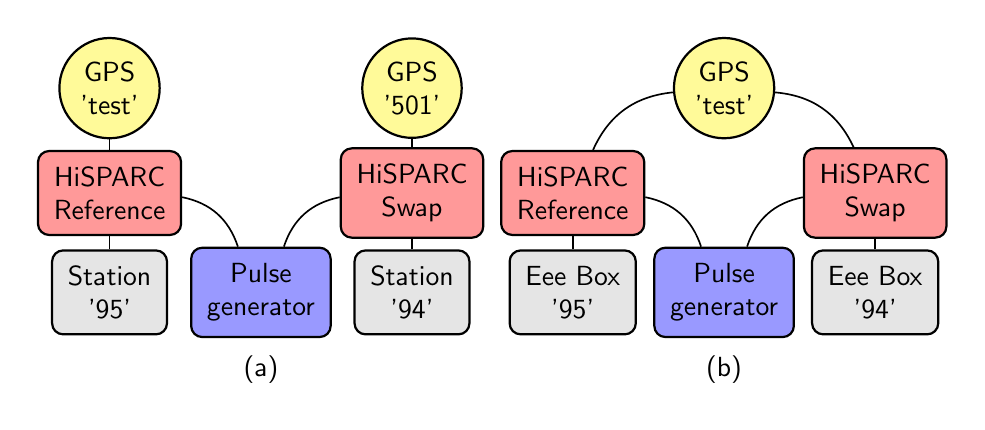
\begin{tikzpicture}
  [font=\sffamily,
   every matrix/.style={ampersand replacement=\&,column sep=0.1cm,row sep=0.1cm},
   gps/.style={draw,thick,circle,fill=yellow!40,inner sep=.1cm, align=center},
   pc/.style={draw,thick,rounded corners,fill=black!10,inner sep=.2cm, align=center},
   hisparc/.style={draw,thick,rounded corners,fill=red!40,inner sep=.2cm, align=center},
   pulse/.style={draw,thick,rounded corners,fill=blue!40,inner sep=.2cm, align=center},
   to/.style={-,semithick,font=\sffamily\footnotesize},]

  \matrix{
   \node[gps] (test) {GPS\\'test'}; \& \& \node[gps] (501) {GPS\\'501'}; \& \& \& \node[gps] (b_test) {GPS\\'test'}; \& \\
   \node[hisparc] (refr) {HiSPARC\\Reference}; \& \& \node[hisparc] (swap) {HiSPARC\\Swap}; \& \& \node[hisparc] (b_refr) {HiSPARC\\Reference}; \& \& \node[hisparc] (b_swap) {HiSPARC\\Swap}; \\
   \node[pc] (95) {Station\\'95'}; \& \node[pulse] (pulse) {Pulse\\generator}; \& \node[pc] (94) {Station\\'94'}; \& \& \node[pc] (b_95) {Eee Box\\'95'};  \& \node[pulse] (b_pulse) {Pulse\\generator}; \& \node[pc] (b_94) {Eee Box\\'94'}; \\
   \& \node {(a)}; \& \& \& \& \node {(b)}; \& \\
  };
  
  \draw[to] (test) -- node[below,above,sloped] {} (refr);
  \draw[to] (501) -- node[below,above,sloped] {} (swap);
  \draw[to] (95) -- node[midway,midway,sloped] {} (refr);
  \draw[to] (94) -- node[midway,midway,sloped] {} (swap);
  \draw[to] (pulse) to[bend left] node[above,below,sloped] {} (swap);
  \draw[to] (pulse) to[bend right] node[above,below,sloped] {} (refr);

  \draw[to] (b_test) to[bend right] node[below,above,sloped] {} (b_refr);
  \draw[to] (b_test) to[bend left] node[below,above,sloped] {} (b_swap);
  \draw[to] (b_95) -- node[midway,midway,sloped] {} (b_refr);
  \draw[to] (b_94) -- node[midway,midway,sloped] {} (b_swap);
  \draw[to] (b_pulse) to[bend left] node[above,below,sloped] {} (b_swap);
  \draw[to] (b_pulse) to[bend right] node[above,below,sloped] {} (b_refr);

 \end{tikzpicture}

    \caption{This image shows the setup of the test, two HiSPARC PCs
             with HiSPARC Masters (Reference and Swap), both connected
             to the same pulse generator. Each is also connected to a
             \gps, some tests used separate \gps antennas (a) and in
             some tests the same \gps was used by both (b).}
    \label{fig:setup}
\end{figure}


\subsection{Offsets between \hisparc electronics}
\label{sub:gps_offsets}

Similar to the offsets between detector pairs within a single stations (see section detector timing) an offset .

Tests to determine the offset distribution between \hisparc electronics have been performed using a \gps splitter to ensure they see the same \gps signal.

Found slightly varying offsets between each \hisparc electronics unit. Constant over time. Can be corrected with enough statistics. Importance of 24 hour self-survey. - Do many 1 hour tests

\todo{Test again year later, same difference??}

The offsets in the \hisparc electronics can be as high as $|\Delta t| = \SI{15}{\ns}$. While the $\sigma_{\Delta t}$ remains within GPS specifications ($\sigma_{\Delta t} < \SI{4.5}{\ns}$).

\todo{Time offset caused by \gps, 501-510 example, \gps swapped}

\gps cable twists affect signal speed?

\begin{figure}
    \centering
    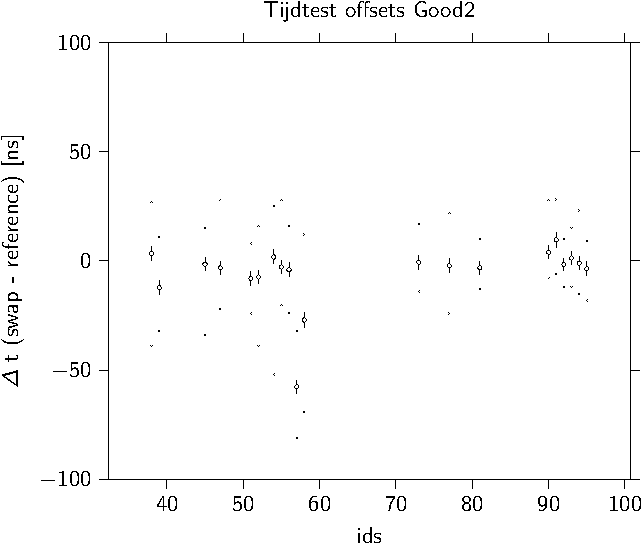
\includegraphics{plots/cluster/hisparc_offsets}
    \caption{Time offsets relative to a reference box. Circles are the
             mean offsets, the error bars the standard deviation and the
             points indicate the minimum and maximum of the test.}
    \label{fig:hisparc_offsets}
\end{figure}


\subsection{Compensating for the offset}

The offset can be determined from real data. For any combination of two stations the expected mean time difference of all coincident events is, because of mirror symmetry, \SI{0}{\ns}. However the spread around the mean is very dependent on the distance between the stations, because showers at an angle will create larger time differences if the stations are further apart. Moreover, the increased distance means that less events will be detected simultaneously by both stations because showers of higher energy and larger footprints occur less often. To determine the offset between stations that are further apart more data is required.

